\documentclass[aspectratio=169,10pt]{beamer}

\usetheme{default}
\usecolortheme{default}
\setbeamertemplate{navigation symbols}{}
\setbeamertemplate{footline}[frame number]
\setbeamertemplate{itemize item}{\textbullet}
\setbeamertemplate{itemize subitem}{\textendash}

% Restrained palette: deep navy, muted teal, warm rust, light gray
\definecolor{LaidlawNavy}{HTML}{1B2A41}
\definecolor{LaidlawTeal}{HTML}{3D6B6E}
\definecolor{LaidlawRust}{HTML}{A85A3A}
\definecolor{LaidlawGray}{HTML}{E8EAED}
\definecolor{LaidlawText}{HTML}{2C2C2C}
\definecolor{LaidlawSoft}{HTML}{F4F6F8}

\setbeamercolor{normal text}{fg=LaidlawText,bg=white}
\setbeamercolor{structure}{fg=LaidlawTeal}
\setbeamercolor{title}{fg=LaidlawNavy}
\setbeamercolor{frametitle}{fg=LaidlawNavy}
\setbeamercolor{subtitle}{fg=LaidlawTeal}
\setbeamercolor{author}{fg=LaidlawText}
\setbeamercolor{date}{fg=LaidlawText}
\setbeamercolor{institute}{fg=LaidlawText}
\setbeamerfont{frametitle}{series=\bfseries,size=\large}
\setbeamerfont{title}{series=\bfseries,size=\LARGE}
\setbeamerfont{subtitle}{size=\large}

\usepackage{booktabs}
\usepackage{graphicx}
\usepackage{microtype}
\usepackage{tikz}
\usetikzlibrary{arrows.meta,positioning,fit,calc,shapes.geometric}
\setlength{\leftmargini}{1.15em}
\setlength{\itemsep}{0.32em}

\newcommand{\statusbox}[3]{%
  \begin{tikzpicture}
    \node[
      draw=#1,
      line width=0.8pt,
      rounded corners=2pt,
      fill=LaidlawSoft,
      align=left,
      text width=0.29\textwidth,
      inner xsep=5pt,
      inner ysep=5pt,
      font=\footnotesize
    ] {%
      {\bfseries\color{#1}#2}\\[0.15em]
      #3%
    };
  \end{tikzpicture}%
}

\title{Temperature and Cardiovascular Admissions in Hong Kong}
\subtitle{HKO exposure file complete; preparing the first HA merge}
\author{Bob Shen}
\date{17 July 2026}
\institute{Laidlaw Scholars Programme}

\begin{document}

%======================================================================
% Frame 1 --- Opening
\begin{frame}[plain]
  \vspace{0.55cm}
  {\color{LaidlawNavy}\LARGE\bfseries Temperature and Cardiovascular Admissions\\[0.15em]
  in Hong Kong\par}
  \vspace{0.45em}
  {\color{LaidlawTeal}\large HKO exposure file complete; preparing the first HA merge\par}

  \vspace{0.85em}
  {\normalsize Bob Shen\\[0.15em]
  Laidlaw Scholars Programme\\[0.15em]
  17 July 2026\par}

  \vspace{1.05em}
  \begin{columns}[T]
    \begin{column}{0.32\textwidth}
      \statusbox{LaidlawTeal}{READY}{132-month HKO exposure file}
    \end{column}
    \begin{column}{0.32\textwidth}
      \statusbox{LaidlawRust}{PENDING}{HA/HPC access and final schema}
    \end{column}
    \begin{column}{0.32\textwidth}
      \statusbox{LaidlawNavy}{TODAY}{Confirm analysis unit, lag plan, and next deliverable}
    \end{column}
  \end{columns}
\end{frame}

%----------------------------------------------------------------------
% Frame 2 --- What is ready for the first merge
\begin{frame}{What is ready for the first merge}
  \begin{columns}[T]
    \begin{column}{0.48\textwidth}
      {\color{LaidlawTeal}\textbf{Completed}}
      \begin{itemize}
        \item HKO Headquarters monthly file, January 2013--December 2023 ($N=132$)
        \item Monthly mean, Tmin, Tmax, and extreme counts
        \item Lag variables constructible
        \item Environmental portion of Table~1 completed
        \item Merge/model pipeline prepared
      \end{itemize}
    \end{column}
    \begin{column}{0.50\textwidth}
      {\color{LaidlawTeal}\textbf{Confirmed by Roro}}
      \begin{itemize}
        \item ICD-9 coding
        \item Complete admission outcomes at patient level
        \item Ages 65--69 and 70--74 available separately
        \item ED-to-inpatient episodes are not included in the extract
        \item HPC onboarding follows wet-ink authorization
      \end{itemize}
    \end{column}
  \end{columns}

  \vspace{0.7em}
  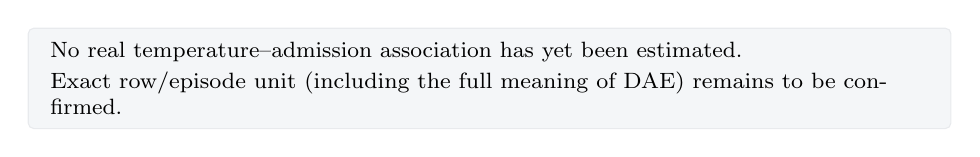
\begin{tikzpicture}
    \node[
      fill=LaidlawSoft,
      draw=LaidlawGray,
      rounded corners=2pt,
      inner xsep=8pt,
      inner ysep=5pt,
      text width=0.92\textwidth,
      align=left,
      font=\footnotesize
    ] {%
      No real temperature--admission association has yet been estimated.\\[0.2em]
      Exact row/episode unit (including the full meaning of DAE) remains to be confirmed.
    };
  \end{tikzpicture}
\end{frame}

%----------------------------------------------------------------------
% Frame 3 --- Environmental exposure visualization
\begin{frame}{Monthly temperature at HKO Headquarters, 2013--2023}
  \begin{center}
    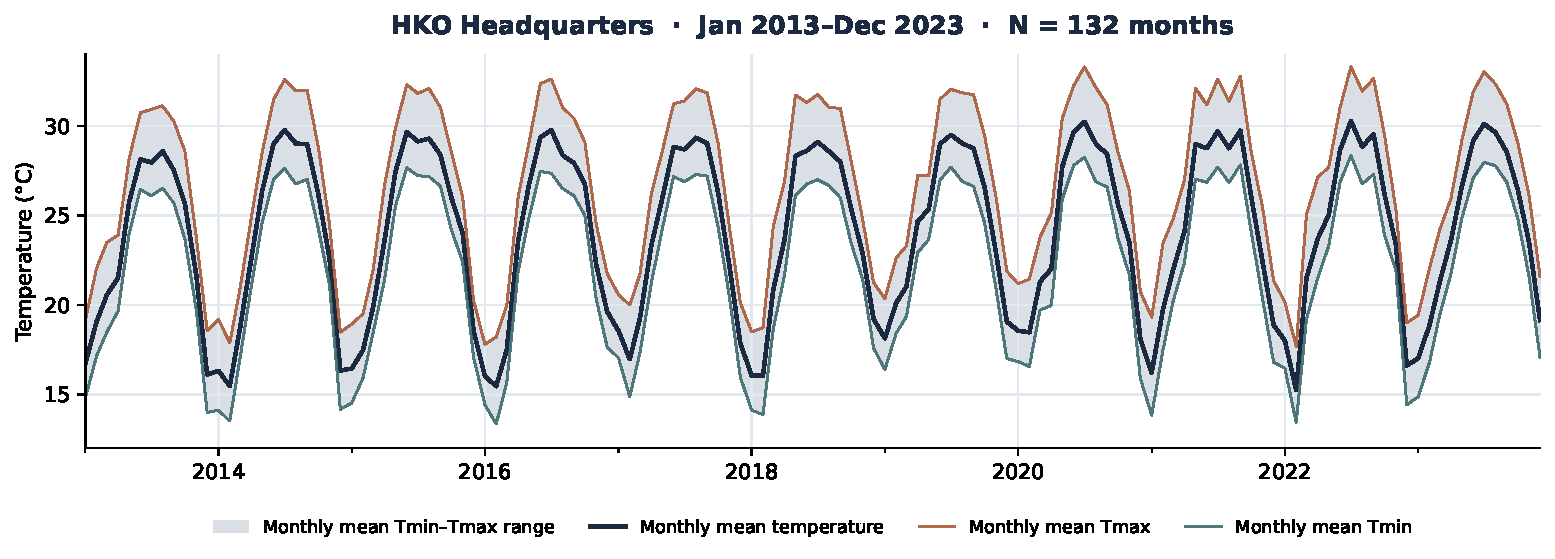
\includegraphics[width=0.93\textwidth]{../../figures/lab_meeting/monthly_temp_ribbon_2013_2023_final.pdf}
  \end{center}
  \vspace{-0.35em}
  \begin{center}
  \scriptsize Environmental exposure data only. Mean with Tmin--Tmax ribbon; $N=132$ months; series ends December 2023.
  \end{center}
\end{frame}

%----------------------------------------------------------------------
% Frame 4 --- Table 1
\begin{frame}{Table 1 is partly complete}
  \begin{columns}[T]
    \begin{column}{0.52\textwidth}
      {\color{LaidlawNavy}\textbf{Panel A --- Environmental observations}}\\[0.15em]
      {\footnotesize Unit: month \quad $N = 132$ months \quad HKO Headquarters}

      \vspace{0.35em}
      \footnotesize
      \begin{tabular}{@{}lrr@{}}
        \toprule
        Variable & Mean & SD \\
        \midrule
        Mean temperature ($^\circ$C) & 24.02 & 4.70 \\
        Mean Tmin ($^\circ$C) & 22.10 & 4.69 \\
        Mean Tmax ($^\circ$C) & 26.66 & 4.82 \\
        Hot nights (days/month) & 3.40 & 5.40 \\
        Very hot days (days/month) & 3.19 & 5.18 \\
        Cold days (days/month) & 1.10 & 2.55 \\
        \bottomrule
      \end{tabular}
    \end{column}
    \begin{column}{0.46\textwidth}
      {\color{LaidlawNavy}\textbf{Panel B --- Patient/admission}}\\[0.15em]
      {\footnotesize Unit and denominator pending confirmation of the HA schema.}

      \vspace{0.35em}
      \footnotesize
      \begin{itemize}
        \item Number of unique patients
        \item Number of qualifying episodes
        \item Age; sex
        \item Diuretics; beta blockers
        \item Metformin; SGLT2 inhibitors
        \item BMI and BMI missingness
      \end{itemize}
    \end{column}
  \end{columns}

  \vspace{0.55em}
  \footnotesize
  These variables can be described as requested; their model role depends on
  the at-risk population and pre-event timing.
\end{frame}

%----------------------------------------------------------------------
% Frame 5 --- Schema question
\begin{frame}{One schema question determines the analysis unit}
  \footnotesize
  Does the extract contain admissions only, or a defined cohort with non-event
  follow-up?

  \vspace{0.55em}
  {\color{LaidlawNavy}\textbf{Proposed default for the first analysis}}
  \vspace{0.25em}

  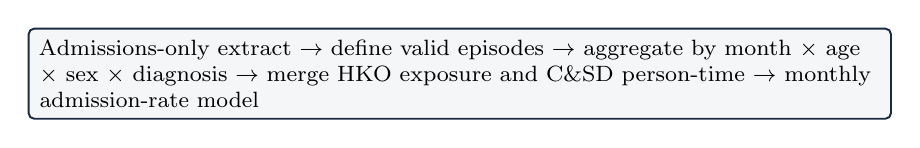
\begin{tikzpicture}[
    node distance=0.22cm,
    box/.style={
      draw=LaidlawNavy,
      line width=0.7pt,
      rounded corners=2pt,
      align=left,
      font=\footnotesize,
      inner sep=4pt,
      text width=0.88\textwidth,
      fill=LaidlawSoft
    },
    arr/.style={-{Latex}, thick, LaidlawTeal}
  ]
    \node[box] (a) {Admissions-only extract
      $\rightarrow$ define valid episodes
      $\rightarrow$ aggregate by month $\times$ age $\times$ sex $\times$ diagnosis
      $\rightarrow$ merge HKO exposure and C\&SD person-time
      $\rightarrow$ monthly admission-rate model};
  \end{tikzpicture}

  \vspace{0.55em}
  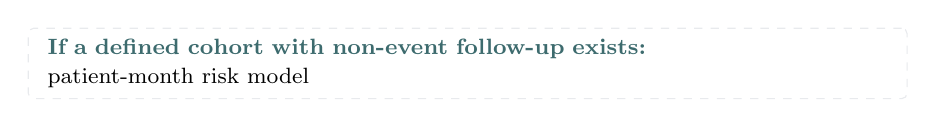
\begin{tikzpicture}
    \node[
      draw=LaidlawGray,
      dashed,
      rounded corners=2pt,
      align=left,
      font=\footnotesize,
      inner xsep=7pt,
      inner ysep=4pt,
      text width=0.88\textwidth,
      fill=white
    ] {%
      {\color{LaidlawTeal}\textbf{If a defined cohort with non-event follow-up exists:}}\\[0.1em]
      patient-month risk model
    };
  \end{tikzpicture}
\end{frame}

%----------------------------------------------------------------------
% Frame 6 --- Temperature and lag specification
\begin{frame}{Temperature variables are ready; proposed first-model sequence}
  \begin{columns}[T]
    \begin{column}{0.46\textwidth}
      \begin{center}
        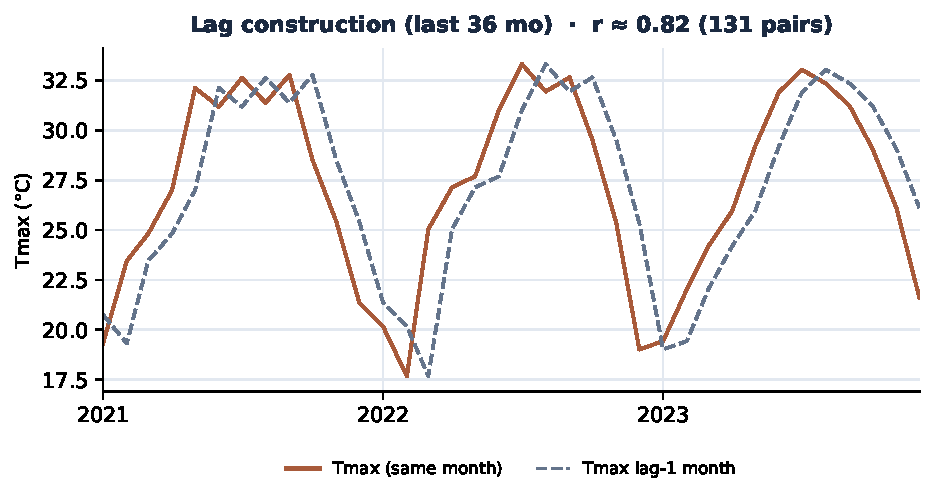
\includegraphics[width=\textwidth]{../../figures/lab_meeting/tmax_lag1_example_final.pdf}
      \end{center}
    \end{column}
    \begin{column}{0.52\textwidth}
      \footnotesize
      \begin{enumerate}
        \item Merge includes contemporaneous and lag-1 mean, Tmin, and Tmax.
        \item Same-month and lag-1 Tmax: $r \approx 0.82$ (131 pairs).
        \item Fit alternative temperature specifications separately.
        \item Proposed sequence:
          \begin{itemize}
            \item same-month exposure (initial)
            \item lag-1 exposure (sensitivity)
            \item current/previous-month average (secondary)
          \end{itemize}
        \item Extend weather input to December 2012 so January 2013 has valid lag-1.
      \end{enumerate}
    \end{column}
  \end{columns}
\end{frame}

%----------------------------------------------------------------------
% Frame 7 --- What needs to be resolved
\begin{frame}{What I need from today's discussion}
  \footnotesize
  \begin{enumerate}
    \item \textbf{Outcome and episode definition}\\[0.1em]
      full meaning of DAE; exact row unit; principal versus any-position diagnosis;
      transfers and recurrent admissions; admission route/elective status.

    \vspace{0.35em}
    \item \textbf{Analysis population}\\[0.1em]
      admissions-only data or defined at-risk cohort;
      availability of medication dates, BMI dates, and non-event follow-up.

    \vspace{0.35em}
    \item \textbf{Access and governance}\\[0.1em]
      wet-ink/HPC timing; whether the expanded work requires an IRB amendment;
      permitted output and disclosure-review process.
  \end{enumerate}

  \vspace{0.45em}
  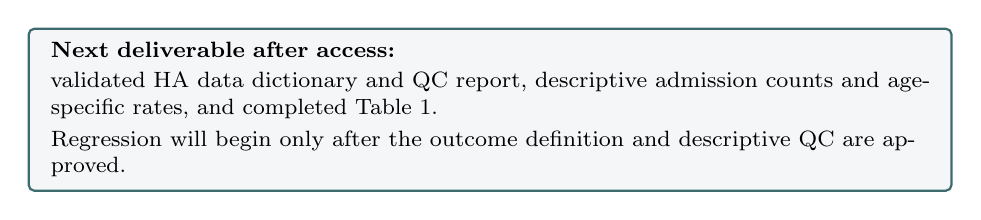
\begin{tikzpicture}
    \node[
      fill=LaidlawSoft,
      draw=LaidlawTeal,
      line width=0.8pt,
      rounded corners=2pt,
      inner xsep=8pt,
      inner ysep=5pt,
      text width=0.92\textwidth,
      align=left,
      font=\footnotesize
    ] {%
      \textbf{Next deliverable after access:}\\[0.15em]
      validated HA data dictionary and QC report,
      descriptive admission counts and age-specific rates,
      and completed Table~1.\\[0.25em]
      Regression will begin only after the outcome definition and descriptive QC
      are approved.
    };
  \end{tikzpicture}
\end{frame}

%======================================================================
\appendix
\begin{frame}[plain]
  \centering
  \vspace{2.4cm}
  {\color{LaidlawNavy}\Large\bfseries Appendix}\\[0.55em]
  {\normalsize Technical detail for discussion if needed}
\end{frame}

%----------------------------------------------------------------------
\begin{frame}{A1. Provisional ICD-9 definitions}
  \footnotesize
  Coding system \textbf{confirmed ICD-9} (Roro, 12~July). Code lists remain provisional
  until principal-diagnosis and local HA rules are confirmed.

  \vspace{0.45em}
  \begin{tabular}{@{}llp{6.0cm}@{}}
    \toprule
    Group & Codes & Notes \\
    \midrule
    AMI & 410.x & Exclude old MI 412 \\
    Hemorrhagic stroke & 430, 431; provisionally 432.x & Sensitivity: 430--431 only \\
    Ischemic stroke & 433.x1, 434.x1, 436 & Sensitivity: with/without 436 \\
    Exclude & 412; 435.x; 438.x & Old MI; TIA; stroke sequelae \\
    \bottomrule
  \end{tabular}

  \vspace{0.55em}
  \scriptsize Source: \texttt{memos/data\_request\_roro.md}. ICD-10 backup retained only if needed historically.
\end{frame}

%----------------------------------------------------------------------
\begin{frame}{A2. Full HKO validation table (annual extremes)}
  \footnotesize
  Station: HKO Headquarters. Result: \textbf{33/33 MATCH} vs HKO \textit{The Year's Weather}.

  \vspace{0.35em}
  \footnotesize
  \begin{tabular}{@{}rrrr@{}}
    \toprule
    Year & Hot nights & Very hot days & Cold days \\
    \midrule
    2013 & 10 & 17 & 14 \\
    2014 & 34 & 33 & 21 \\
    2015 & 37 & 28 & 7 \\
    2016 & 36 & 38 & 21 \\
    2017 & 41 & 29 & 9 \\
    2018 & 26 & 36 & 21 \\
    2019 & 46 & 33 & 1 \\
    2020 & 50 & 47 & 11 \\
    2021 & 61 & 54 & 13 \\
    2022 & 52 & 52 & 13 \\
    2023 & 56 & 54 & 14 \\
    \bottomrule
  \end{tabular}

  \vspace{0.4em}
  \scriptsize Source: \texttt{outputs/tables/hko\_annual\_extremes\_validation.csv}.
\end{frame}

%----------------------------------------------------------------------
\begin{frame}{A3. Detailed HA schema questions}
  \footnotesize
  \begin{enumerate}
    \item What does ``DAE records included'' mean in this ICD-9 extract? (No expansion invented.)
    \item Is each row one admission episode, with drugs/BMI attached if available?
    \item Can principal diagnosis be distinguished from secondary diagnoses?
    \item Which admission-route or elective/emergency fields are available?
    \item How are inter-hospital transfers and same-patient recurrence handled?
    \item Are diuretics, beta blockers, metformin, SGLT2is, and BMI already on the approved extract?
    \item What medication and BMI measurement dates are available relative to admission?
    \item Does the extract contain non-event follow-up / a defined at-risk cohort, or admissions only?
    \item What small-cell suppression rules apply to descriptive outputs from HPC?
  \end{enumerate}
\end{frame}

%----------------------------------------------------------------------
\begin{frame}{A4. Pipeline / data flow}
  \footnotesize
  \begin{center}
  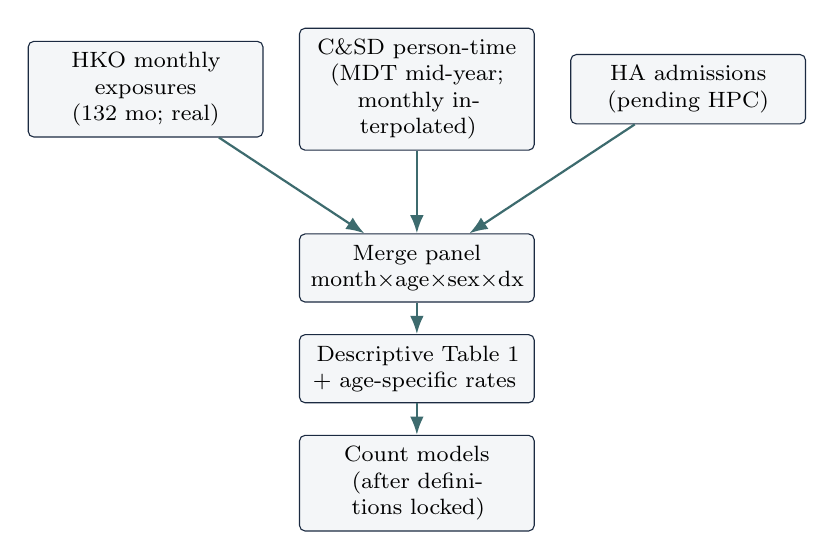
\begin{tikzpicture}[
    node distance=0.4cm and 0.45cm,
    box/.style={draw=LaidlawNavy, rounded corners=2pt, align=center, font=\footnotesize,
      inner sep=4pt, text width=2.7cm, fill=LaidlawSoft},
    arr/.style={-{Latex}, thick, LaidlawTeal}
  ]
    \node[box] (hko) {HKO monthly exposures\\(132 mo; real)};
    \node[box, right=of hko] (csd) {C\&SD person-time\\(MDT mid-year;\\monthly interpolated)};
    \node[box, right=of csd] (ha) {HA admissions\\(pending HPC)};
    \node[box, below=1.05cm of csd] (merge) {Merge panel\\month$\times$age$\times$sex$\times$dx};
    \node[box, below=of merge] (desc) {Descriptive Table~1\\+ age-specific rates};
    \node[box, below=of desc] (mod) {Count models\\(after definitions locked)};
    \draw[arr] (hko) -- (merge);
    \draw[arr] (csd) -- (merge);
    \draw[arr] (ha) -- (merge);
    \draw[arr] (merge) -- (desc);
    \draw[arr] (desc) -- (mod);
  \end{tikzpicture}
  \end{center}

  \vspace{0.35em}
  \scriptsize
  Scripts: \texttt{02\_build\_weather\_monthly.R}, \texttt{05\_build\_population\_denominators.R},
  \texttt{08b\_merge\_real\_ha\_panel.R}. Synthetic track exists only for workflow testing --- not findings.\\
  Population status: \texttt{CSD\_IMPORTED} from Table 110-01001; monthly values are interpolated.
\end{frame}

%----------------------------------------------------------------------
\begin{frame}{A5. Full Table~1 shell}
  \footnotesize
  \textbf{Panel A --- filled} ($N=132$ months; HKO Headquarters)\\[0.2em]
  Mean temp 24.02 (4.70)~$^\circ$C; Tmin 22.10 (4.69)~$^\circ$C; Tmax 26.66 (4.82)~$^\circ$C;
  hot nights 3.40 (5.40); cold days 1.10 (2.55); very hot days 3.19 (5.18).

  \vspace{0.5em}
  \textbf{Panel B --- pending HA access}\\[0.2em]
  \begin{tabular}{@{}lp{8.8cm}@{}}
    \toprule
    Field & Status / note \\
    \midrule
    $N$ patients / episodes & Pending; denominator depends on schema \\
    Age, sex & Requested; strata include 65--69 and 70--74 \\
    Diuretics; beta blockers & Requested descriptively; model role TBD \\
    Metformin; SGLT2 inhibitors & Requested descriptively; model role TBD \\
    BMI (+ missingness) & Requested descriptively; pre-event timing TBD \\
    \bottomrule
  \end{tabular}

  \vspace{0.4em}
  \scriptsize
  These covariates will be described as requested. Model use depends on cohort structure and measurement timing.
\end{frame}

%----------------------------------------------------------------------
\begin{frame}{A6. Deferred pollution, district, and 2024 extensions}
  \footnotesize
  \begin{itemize}
    \item \textbf{Pollution:} EPD import scripts ready; current file is a placeholder
      (\texttt{PLACEHOLDER\_NOT\_FOR\_INFERENCE}). Near-term priority remains
      temperature $\rightarrow$ AMI/stroke after HA access.
    \item \textbf{District / multi-station weather:} HKO Headquarters is the primary
      station. Multi-station or district extensions are optional sensitivities (Hogan),
      not required for the first HA report.
    \item \textbf{2024 weather extension:} Optional; raw 2024 extract exists.
      Do not delay the 2013--2023 HA core.
  \end{itemize}
\end{frame}

\end{document}
